\documentclass[xcolor=dvipsnames]{beamer}
\usepackage{epstopdf}
\usepackage[german]{babel}
\usepackage[utf8]{inputenc}
\usepackage[procnames]{listings}
\usepackage{color}
\usepackage[lined, boxed, commentsnumbered, linesnumbered]{algorithm2e}
\usepackage{xfrac}
\usepackage{pgfplots}
\usepackage{tikz}
\tikzset{
    declare function={Floor(\x)=round(\x-0.5);}
}
\tikzset{
    declare function={Ceil(\x)=round(\x+0.5);}
}

\renewcommand*{\algorithmcfname}{Algorithmus}
\makeatletter
\newcommand*{\rom}[1]{\expandafter\@slowromancap\romannumeral #1@}
\makeatother
\usetheme{Madrid}

%\setbeamertemplate{itemize items}[square]
\beamertemplatenavigationsymbolsempty
%\setbeamersize{text margin left=1cm,text margin right=1cm}

\title{TranscriptionDesk}
\subtitle{a Citizen Science Project}
\author{R. Rößling, J. Runge, O. Schurig, F. Teichmann}
\institute{University of Leipzig}
\date{15. July 2015}

\begin{document}
\frame{\titlepage}
\frame{\tableofcontents}

\section{Introduction}
\begin{frame}{Introduction}
    \begin{itemize}
        \item Platform to transcribe historical texts.
        \item Historical manusscripts have been scanned.
        \item OCR is not possible.
        \\$\Rightarrow$ Citizen Science can help here.
    \end{itemize}
\end{frame}
\section{Project plan}
\begin{frame}{Project plan}
    \begin{itemize}
        \item Agile software development model.
        \item First Milestone:
        \begin{itemize}
            \item User authentication logic \checkmark
            \item Database mockup \checkmark
            \item Interface mockup \checkmark
            \item Omeka Service Provider \checkmark
        \end{itemize}
        \item Second Milestone:
        \begin{itemize}
            \item Storage and voting for areas of interest.
            \item MUFI input system.
            \item …
        \end{itemize}
        \item Third Milestone:
        \begin{itemize}
            \item Completion of System
            \item Eventual bugfixes
        \end{itemize}
    \end{itemize}
\end{frame}
\section{Architecture}
\begin{frame}{Components}
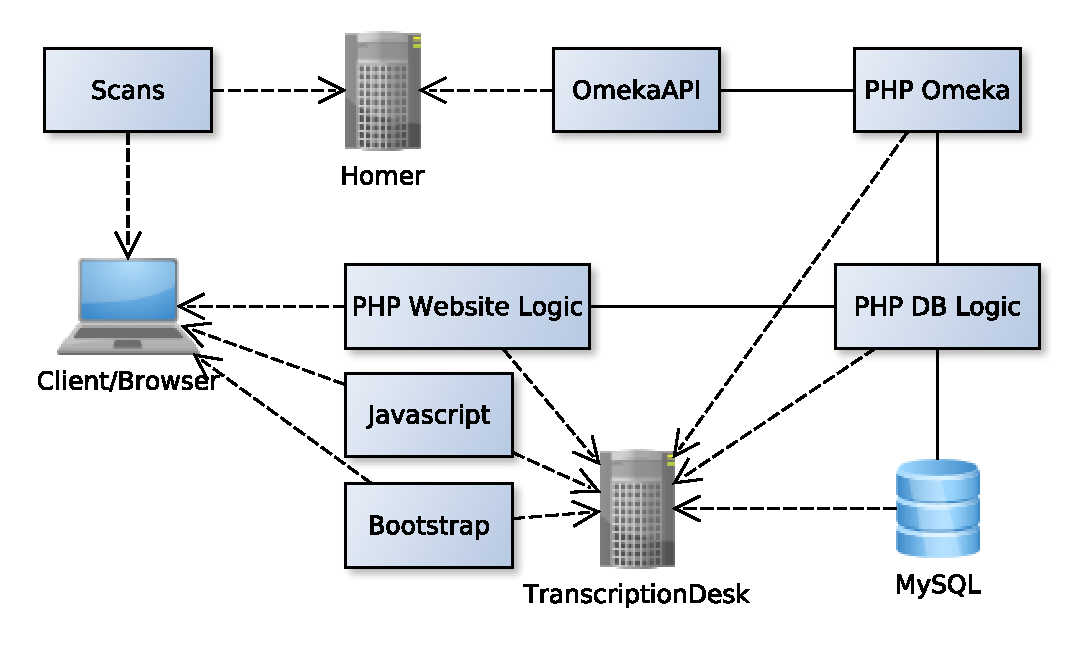
\includegraphics[width=\textwidth]{./components.pdf}
\end{frame}
\begin{frame}{Database}
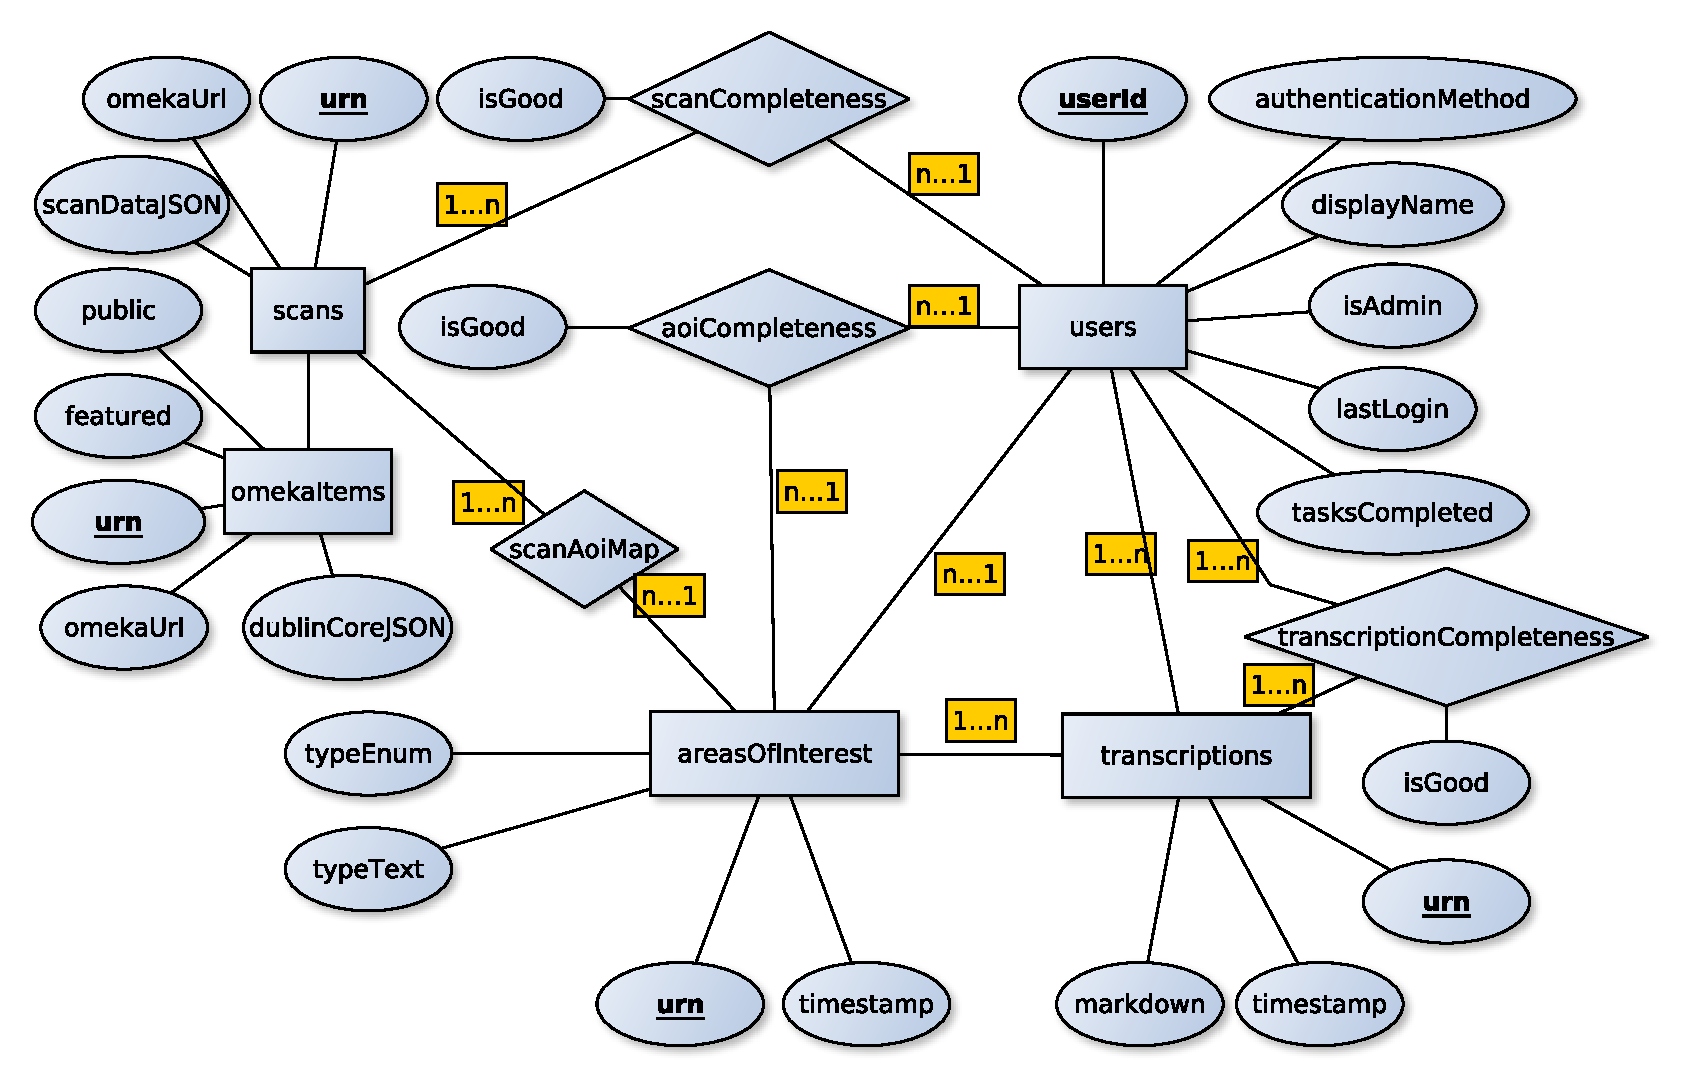
\includegraphics[width=\textwidth]{./ER.pdf}
\end{frame}
\begin{frame}{Technologies}
    \begin{itemize}
        \item LAMP setup
        \item Omeka
        \item Opauth
        \item GitHub
        \item jQuery
        \item OpenLayers
        \item ACE
        \item To come: MUFI, Markdown rendering, …
    \end{itemize}
\end{frame}
\section{Live demo}
\begin{frame}{Live demo}
    Let's look at the Website!
\end{frame}
\end{document}
